\documentclass{article}
\usepackage[utf8]{inputenc}
\usepackage{amsmath}
\usepackage{float}
\usepackage{tikz}
\usetikzlibrary{arrows.meta,positioning}

\title{Mathematical Modelling in \LaTeX}
\author{Gurobi Optimization}

\begin{document}

\maketitle

This document provides an example of how \LaTeX\ can be used to write clean mathematical models. As an example, we consider the famous maximum flow / minimum cut problems. The problems consider a directed graph consisting of a set of nodes and a set of labeled arcs. The arc labels are non-negative values representing a notion of capacity for the arc. In the node set, there exists a source node $s$ and a terminal node $t$. The amount of flow into one of the intermediary nodes must equal the amount of flow out of the node, i.e., flow is conserved. 

The maximum flow question asks: what is the maximum flow that can be transferred from the source to the sink. The minimum cut question asks: which is the subset of arcs, that once removed would disconnect the source node from the terminal node, which has the minimum sum of capacities. For example, removing arcs $(v_1, v_3)$ and $(v_2, v_4)$ from the network in \ref{fig:my_label} would mean there is no longer a path from $s$ to $t$ and the sum of the capacities of these arcs is $12 + 11 = 23$. It is reasonably straight forward to find a better cut, i.e., a subset of nodes with sum of capacities less than 23.


% Image courtesy of https://tex.stackexchange.com/questions/341949/how-to-plot-a-network-flow-with-tikz

\begin{figure}[H]
    \centering
    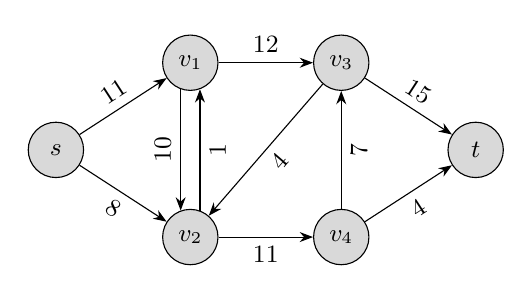
\begin{tikzpicture}[
      mycircle/.style={
         circle,
         draw=black,
         fill=gray,
         fill opacity = 0.3,
         text opacity=1,
         inner sep=0pt,
         minimum size=20pt,
         font=\small},
      myarrow/.style={-Stealth},
      node distance=0.6cm and 1.2cm
      ]
      \node[mycircle] (c1) {$s$};
      \node[mycircle,below right=of c1] (c2) {$v_2$};
      \node[mycircle,right=of c2] (c3) {$v_4$};
      \node[mycircle,above right=of c1] (c4) {$v_1$};
      \node[mycircle,right=of c4] (c5) {$v_3$};
      \node[mycircle,below right=of c5] (c6) {$t$};

    \foreach \i/\j/\txt/\p in {% start node/end node/text/position
      c1/c2/8/below,
      c1/c4/11/above,
      c2/c3/11/below,
      c3/c6/4/below,
      c4/c5/12/above,
      c5/c6/15/above,
      c5/c2/4/below,
      c3/c5/7/below,
      c2.70/c4.290/1/below}
       \draw [myarrow] (\i) -- node[sloped,font=\small,\p] {\txt} (\j);


     % draw this outside loop to get proper orientation of 10
     \draw [myarrow] (c4.250) -- node[sloped,font=\small,above,rotate=180] {10} (c2.110);
    \end{tikzpicture}
    \caption{Example network}
    \label{fig:my_label}
\end{figure}




A complete model is provided for the maximum flow problem, whereas the minimum cut problem is left as a challenge to the reader.

\section*{Notation}

\subsection*{Sets}

\begin{table}[H]
\centering
\begin{tabular}{p{1cm} p{1.5cm} p{9cm}}
\hline
\textbf{Index} & \textbf{Set} & \textbf{Description}\\
\hline
$i$ & $V$ & Set of all nodes ($s$ source and $t$ terminal)\\
$(i, j)$ & $A$ & Set of all arcs\\
\hline
\end{tabular}
\end{table}

\subsection*{Parameters}

\begin{table}[H]
\centering
\begin{tabular}{p{2cm} p{9cm}}
\hline
\textbf{Parameter} &  \textbf{Description}\\
\hline
$c_{i,j}$ & Capacity of arc $(i,j) \in A$\\
\hline
\end{tabular}
\end{table}

\section*{Maximum Flow}


\subsection*{Variables}

\begin{table}[H]
\centering
\begin{tabular}{p{2cm} p{1.5cm} p{9cm}}
\hline
\textbf{Variable} & \textbf{Type}& \textbf{Description}\\
\hline
$f_{i, j}$ & Cont & flow from $i$ to $j$ in arc $(i,j) \in A$\\
\hline
\end{tabular}
\end{table}

\subsection*{Model}

\begin{subequations}
\begin{alignat}3
\text{maximise} \ & \sum_{j \in V: (s,j) \in A} f_{s, j} \label{model-obj}\\
s.t. \ & f_{i, j} \leq c_{i,j} \quad && \forall (i, j) \in A \label{m1-c1}\\
& \sum_{i \in V: (i,j) \in A} f_{i, j} - \sum_{k \in V: (j, k) \in A} f_{j,k} = 0 \quad  && \forall j \in V \setminus \{s, t\} \label{m2-c2}
\end{alignat}
\end{subequations}

The objective \eqref{model-obj} is to maximise the sum of flow leaving the source node $s$. Constraints \eqref{m1-c1} ensure that the flow in each arc does not exceed the capacity of that arc. Constraints \eqref{m2-c2} are continuity constraints, which ensure that the flow into each of the nodes, excluding the source and sink, is equal to the flow out of that node.

\newpage

\section*{Minimum Cut}

This section is left for the reader to complete


\subsection*{Variables}

\begin{table}[H]
\centering
\begin{tabular}{p{2cm} p{1.5cm} p{9cm}}
\hline
\textbf{Variable} & \textbf{Type}& \textbf{Description}\\
\hline
$r_{i, j}$ &  & 1 if arc $(i,j) \in A$ is removed\\
$z_{i, j}$ &  & 1 if node $i \in V \setminus \{s, t\}$ connected to $s$, 0 otherwise\\
\hline
\end{tabular}
\end{table}

\subsection*{Model}

\begin{subequations}
\begin{alignat}3
\text{to do} 
\end{alignat}
\end{subequations}


\end{document}
